\documentclass[border=2pt]{standalone}
\usepackage{amsmath}
\usepackage{tikz}
\usetikzlibrary{matrix,decorations.pathreplacing,calc,positioning}

% Row-brace (left side, labels the row count) and column-underbrace (bottom,
% labels the column count) for a tikz "matrix of math nodes" named #1,
% labeled #2 (rows) and #3 (cols).
\newcommand{\rowbrace}[3]{%
  \draw[decorate,decoration={brace,amplitude=6pt,mirror}]
    ($(#1.north west)+(-4pt,0)$) -- ($(#1.south west)+(-4pt,0)$)
    node[midway,left=8pt] {$#2$};
  \draw[decorate,decoration={brace,amplitude=6pt,mirror}]
    ($(#1.south west)+(0,-4pt)$) -- ($(#1.south east)+(0,-4pt)$)
    node[midway,below=8pt] {$#3$};
}

\begin{document}
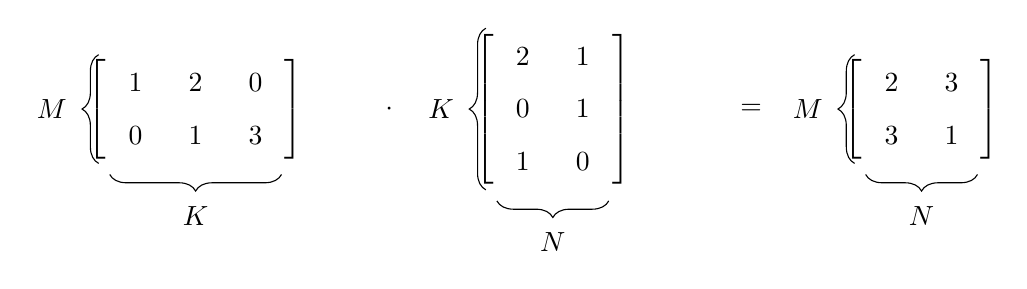
\begin{tikzpicture}[baseline=(current bounding box.center)]

  \matrix (A) [matrix of math nodes, left delimiter={[}, right delimiter={]},
               column sep=10pt, row sep=6pt, ampersand replacement=\&] {
    1 \& 2 \& 0 \\
    0 \& 1 \& 3 \\
  };
  \rowbrace{A}{M}{K}

  \node[right=34pt of A] (dot) {$\cdot$};

  \matrix (B) [matrix of math nodes, left delimiter={[}, right delimiter={]},
               column sep=10pt, row sep=6pt, ampersand replacement=\&,
               right=34pt of dot] {
    2 \& 1 \\
    0 \& 1 \\
    1 \& 0 \\
  };
  \rowbrace{B}{K}{N}

  \node[right=44pt of B] (eq) {$=$};

  \matrix (C) [matrix of math nodes, left delimiter={[}, right delimiter={]},
               column sep=10pt, row sep=6pt, ampersand replacement=\&,
               right=34pt of eq] {
    2 \& 3 \\
    3 \& 1 \\
  };
  \rowbrace{C}{M}{N}

\end{tikzpicture}
\end{document}
